% CAPITULO 1: EXPLICO EL ESQUEMA GENERAL DEL ALGORITMO

\chapter{Herramienta desarrollada}
\label{method}


\section{Fundamentos del método utilizado}
\label{fundamentos}

\subsection{Detección de propiedades a partir del análisis secuencial}

% Mapeo de los objetivos con existencia de herramientas disponibles.

% PRIMERO QUE BUSCAMOS EN REALIDAD
% Para entender los fundamentos del método implementado primero debemos analizar mejor los detalles del objetivo.
% El requerimiento fundamental de la secuencia linker resultante es que esta posea la flexibilidad necesaria para que los dominios que conecta se muevan libremente.
% Para poder lograr esto la secuencia debe adoptar y mantener \textit{in-vivo} las características de un amplio ensamble conformacional que no restrinja la estructura, 
% lo cual está asociado a las propiedades conformacionales de las proteínas intrínsecamente desordenadas. 
% % donde las diferentes conformaciones desordenadas se intercambian rápidamente de manera continua 
% % Por lo tanto, tenemos un panorama mas claro acerca de cuales serán las características conformacionales de la secuencia que esperamos obtener.
% Como se detalló en la introducción,  han permitido comprender cuales son las características que distinguen a estos elementos proteicos. 
% Las propiedades estudiadas sirven para implementar una gran cantidad de herramientas bioinformáticas capaces de distinguir es



% 
% 
% % Como vimos en la sección \ref{linkerDesign} la flexibilidad no es todo y, por eso, 
% Otra parte fundamental del objetivo es que el linker obtenido se mantenga inerte frente a cualquier actividad biológica que pueda 
% interferir en el proceso se expresión o en la correcto funcionamiento de la proteína resultante del diseño.
% % Una parte relevante de esta secuencia objetivo es su inercia frente al pipeline de 
% En la sección \ref{functionalLandscape} se describieron distintos elementos funcionales que pueden estar presentes en una secuencia.
% Clasificando, aislando y analizando estos elementos hemos podido comprender mejor cuales son sus propiedades. 
% Lo que lo objetivo requiere, entonces, es que la secuencia resultante este libre de cualquiera de estos elementos permaneciendo, preferentemente, inerte ante cualquier actividad o interacción posible \textit{in-vivo}.
% 
% % Teniendo en claro los objetivos en términos de los posibles elementos estructurales y funcionales, lo que el método requiere es, entonces, obtener una secuencia que adopte ,que esté limpia de elementos estructurales 
% A lo largo del capítulo 1, hemos presentado una gran cantidad de conocimientos obtenidos acerca de las propiedades secuenciales y su relación con la conformación y función resultante.
% Los avances mostrados en este campo se trasladan a una gran cantidad(y variedad) de métodos que permiten predecir la ocurrencia de estas propiedades sobre cualquier secuencia polipeptídica.





En la sección \ref{aspectosDiseno} se desarrollaron distintos aspectos estucturales y funcionales que se deben tener en cuenta en el diseño de un linker.
A partir de esta descripción podemos distinguir claramente diferentes características que afectan positiva y negativamente a la funcionalidad del diseño resultante.
Esto permite definir una secuencia linker como aquella que posea todas las característica positivas y no posea ninguna de las característica negativas buscadas.
Es importante recordar que, como se describió previamente, algunas de las características están en función de consideraciones hechas por el usuario experimental.

En la sección \ref{modulosProteicos} describimos distintos módulos proteicos encontrados en la naturaleza, identificando los elementos conformacionales y funcionales asociados.
El estudio de estos elementos generalmente apunta, no sólo a modelizar sus propiedades asociadas (macanismos funcionales, estructuras, propiedades secuenciales asociadas, etc.), 
sino también a poder trasladar los conocimientos en herramientas bioinformáticas que permitan predecir la ocurrencia de estos.
Estas propiedades están directamente asociadas a la secuencia de la proteína, además, la secuencia es lo primero que se conoce cuando se encuentra o diseña una nueva proteína, por lo tanto,  
como objetivo general se intenta poder obtener la mayor cantidad de información a partir de ésta.
Como consecuencia, existen cada vez más herramientas, que utilizando aproximaciones distintas, las cuales permiten detectar un diverso perfil de características a partir de la secuencia.

% Como vimos en la sección \ref{modulosProteicos} estas características están asociadas a distintos elementos proteicos estudiados a partir de su ocurrencia en proteínas naturales.
% Los elementos estructurales y funcionales y su  
% Todas estas características estructurales y funcionales han sido estudiadas en el contexto de los módulos proteicos encontrados en proteinas naturales.
% los cuales se muestran en las primeras secciones de este capitulo.
% Como vimos en la sección \ref{modulosProteicos}, los distintos elementos conocimientos obtenidos permiten comprender los aspectos      y cómo 
% Los conocimientos obtenidos(desarrollados en la sección \ref{modulosProteicos}) permiten, no sólo entender estas propiedades, sino también desarrollar 
% diferentes herramientas bioinformáticas utilizadas luego para predecir la ocurrencia de estas propiedades a partir de la secuencia polipeptídica.
% Los estudios han resultado en un amplio conocimiento de las propiedades secuenciales y 
% Los avances en este campo se trasladan a una gran cantidad de métodos que, a través de diferentes aproximaciones, permiten predecir estas propiedades a partir de la secuencia polipeptídica.

Una parte fundamental del método implementado en este trabajo es que actualmente podemos predecir, con cierta probabilidad, 
la ocurrencia de los distintos aspectos positivos y negativos asociados a un linker conociendo solamente la secuencia de aminoácidos de una proteína.
% Esto tiene como corolario que podremos decir si una secuencia resultará o no en un buen candidato para funcionar como linker, usando estas Usando la definición de linker que recien vimos parametrizadas con las características que , 
Lo que es más, las predicciones pueden ser mapeadas a posiciones puntuales que actúan favoreciendo a las distintas características dentro de la secuencia. 
Por ejemplo, podemos mapear dentro de la secuencia cuales serán las posiciones 
que favoreceran la adopción de una conformación intrínsecamente desordenada, lo cual es una característica deseable para el diseño de un linker.







\subsection{Espacio de secuencias buscadas}\label{espacioSecuencial}

% *****************PROPIEDADES DEL ESPACIO DE BUSQUEDA 

% las propiedades conformacionales pueden ser un especto muy importante si se intenta diseñar proteínas con estructura plegada definida
De todos los requerimientos de diseño vistos en la sección \ref{aspectosDiseno} el más restrictivo es, en principio, que el diseño resultante tenga con la flexibilidad necesaria. 
Esto implica que la secuencia se ajuste a las propiedades de una proteína intrínsecamente desordenada, las cuales identificamos previamente como un conjunto de secuencias 
claramente sesgadas en su composición, con baja complejidad y generalmente desprovistas de varios tipos de aminoácidos.
Esto parece indicar que el espacio de secuencias comprendido por éstas debe ser significativamente pequeño con respecto al espacio total de posibles soluciones(todas las posibles combinaciones de aminoácidos),
y por lo tanto obtener un diseño que encaje dentro de este espacio deja pocas opciones y hace difícil la búsqueda de la secuencia resultante.

Sin embargo, la realidad es mas compleja de lo que parece.
Las IDPs no requieren que su secuencia posea un código definiendo el plegamiento y la estructura nativa final. 
Además, vimos que las IDPs se caracterizan por tener secuencias conteniendo múltiples elementos estructurales y funcionales relativamente cortos, formando un mosaico 
De esta forma, el espacio abarcado por las secuencias que poseen las propiedades conformacionales que buscamos, puede no es tan restringido como se pensabamos y, de hecho,
puede tener un tamaño considerable con respecto al espacio total de posibles soluciones.
Dentro de este espacio, el resto de las propiedades positivas que buscamos y de las propiedades negativas que queremos evitar, no restringe demasiado el número de soluciones
ya que, como vimos, probablemente esten limitadas a segmentos muy cortos sobre la secuencia.

Asumimos, entonces, que el conjunto de diseños posibles, constituido por todas las secuencias que poseen las propiedades positivas y 
no poseen las negativas, tiene un tamaño considerable con respecto al espacio de posibles soluciones compuesto por todas las combinaciones de aminoácidos.
Este conjunto, sin embargo, pude reducirse considerablemente si se tienen en cuenta algunos aspectos definidos por el usuario 
como una composición secuencial muy especifica, una carga neta elevada, o una combinación de cualquiera de éstos. 















\section{Esquema general de la implementación}




% De esta forma, estamos en una situación en la que: tenemos un conjunto de herramientas que nos permiten mapear cada secuencia con distintos comportamientos (deseado o no deseados) de acuerdo a nuestros objetivos y, además, 
% podemos asumir que el conjunto de secuencias que cumple con los principales comportamientos buscados es considerablemente grande con respecto al espacio de soluciones posibles (cualquier combinación de AAs).



A partir de los aspectos detallados en los fundamentos, una primera aproximación obvia sería realizar una búsqueda sistematica dentro del espacio 
de secuencias hasta obtener una que resulte favorable de acuerdo a nuestros parámetros de evaluación.  
El problema radica en que es una forma totalmente ineficiente de búsqueda, tiene un alto costo computacional y el resultado(asumiendo que lo encontramos) será una composición al azar.
Una aproximación mas adecuada,  sería utilizar todo el conocimiento que tenemos para poder evaluar la secuencia y usar esto a nuestro favor para guiar la búsqueda. 
Al guiar la búsqueda utilizando los resultados de las evaluaciones, esta sera mucho mas efectiva y el costo computacional sera mucho menor.
Además, según el punto de inicio que utilicemos para la búsqueda, podremos intentar obtener secuencias resultantes con cierta similitud.

% La existencia de una función ideal implicaría que esta represente la dependencia de cada posicion con el contexto de la secuencia, con respecto a la propiedad analizada.
% Si bien las herramientas disponibles de predicción nos son las ideales, generalmente brindan información sobre cada posición y no sobre la secuencia como un todo.

% Uilizando esta información podríamos analizar que posiciones no son acordes con el comportamiento/propiedades deseado/a y utilizar esta información para guiar la búsqueda, modificando solo aquellas posiciones que no nos resultan favorables.
 
% Si bien asumimos que el conjunto de secuencia que cumplen las condiciones estandar del resultado es grande con respecto al especio total de soluciones, no conocemos la forma funcional que no esta guiando la busqueda,
% es decir, como esta depende con la secuencia.  Para implementar un mecanismo eficiente de búsqueda debemos tener en cuenta este desconocimiento.

El procedimiento general del algoritmo consiste en aplicar mutaciones puntuales iterarativamente a partir de una secuencia inicial, en busca de la secuencia final con las características deseadas.
En cada iteración se proponen y analizan posibles mutaciones de acuerdo a un sistema de evaluación de secuencias.
La selección de posibles posiciones a mutar se hace de acuerdo a un muestreo ponderado en función de los resultados de la evaluación secuencial.
Además, la aceptación de cada mutación está asociada a un método heurístico de decisión.
De esta forma, la secuencia de mutaciones aceptadas para una determinada secuencia inicial no necesariamente será siempre la misma, 
la búsqueda será guiada por el análisis realizado sobre las secuencias pero no quedará completamente determinada por éste. 

En la figura \ref{fig:esquema-algoritmo} se ve un esquema general del método completo. 
En la seccion \ref{seqInicial} se detalla como se obtiene la secuencia inicial y luego en las secciones \ref{evaluacion} y \ref{mutacion} se describen y ejemplifican los pasos para evaluar la secuencia y obtener una mutación puntual 
en cada iteración.


\begin{figure}[h!]
\centering
   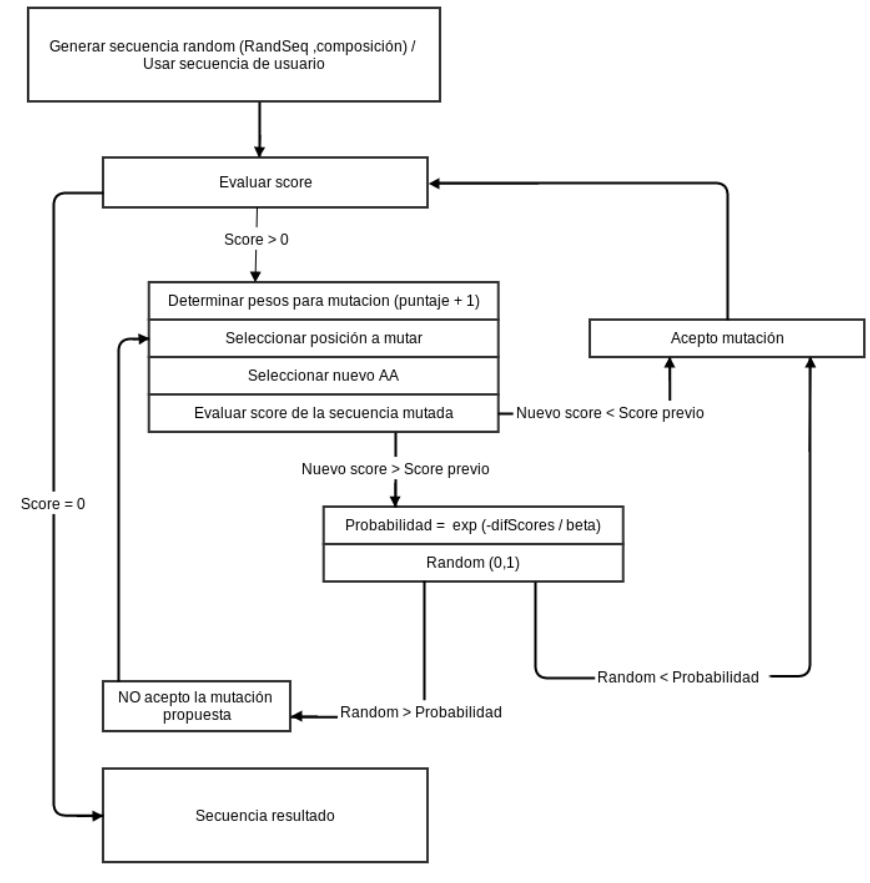
\includegraphics[width=\textwidth]{img/diagrama-algoritmo-2.png}
 \caption{Esquema general del método aplicado para obtener la secuencia final}
 \label{fig:esquema-algoritmo}
\end{figure}

El resultado principal de la ejecución es una secuencia que cumple con todas las características positivas que se indicaron y no posee ninguno de los aspectos negativos.
En un archivo asociado se refleja el proceso de mutación indicando, para cada paso, cual es la posición mutada y la secuencia resultante.
Otras opciones de salida son posibles, en la sección \ref{output} del manual se describen opciones que permiten, entre otras cosas, realizar una ejecución paso o a paso con detalles de cada evaluación realizada, 
o limitar la salida mostrando unicamente la secuencia resultante.

\subsection{Secuencia inicial}\label{seqInicial}

El método comienza a iterar a partir de una secuencia inicial. 
Esta secuencia puede ser creada de forma aleatoria como primer paso del 
algoritmo(ver \ref{secuenciaInicialRandom}) o puede ser pasada como parámetro por el usuario \ref{secuenciaInicialDefinida}. 

En el caso que se defina una secuencia inicial esta definirá también, de manera implícita, la logitud de la secuencia resultante. Por lo tanto, no es necesario definir la longitud.
Sin embargo, en este caso se da la posibilidad al usuario de identificar segmentos flanqueantes en uno o ambos extremos de esta secuencia inicial que, si bien serán tenidos en cuenta a la hora de la evaluación,
no serán mutados como parte del proceso y por lo tanto formarán parte del diseño resultante. 
La utilización de esta parametrización opcional se detalla en la sección \ref{flanqueantes} del manual.

La generación de una secuencia aleatoria no es un problema trivial. 
En la naturaleza las proteínas están compuestas de un conjunto de 20 aminoácidos, los cuales se encuentran con diferentes abundancias relativas. 
La frecuencia de cada aminoácido dentro de un proteoma está dada por un balance entre el costo metabólico de este y la necesidad de contar con un conjunto de secuencias diversas que darán proteínas funcionales \cite{krick2014amino}. 
Para generar una secuencia aleatoria, entonces, es necesario definir primero la frecuencia que tendrá cada aminoácido. 
Esta frecuencia se obtiene a partir de la frecuencia global que tiene cada aminoácido en la base de datos de secuencias proteicas.
La aplicación que se utiliza para obtener la secuencia random es RandSeq \cite{randseq}.

Por default, la herramienta utiliza la composición estándar obtenida de SwissProt \cite{compositionAA}.  
Estos valores resultan del cálculo de la composición de aminoácidos de todas las proteínas de la base de datos. 
De esta forma, la composición total representa un consenso de frecuencias de aminoácidos entre todas las secuencias documentadas hasta el momento en la base de datos UniProtKB/Swiss-Prot.
% Los valores de la composición estándar se encuentran en http://web.expasy.org/protscale/pscale/A.A.Swiss-Prot.html

Entre otras que existen, esta herramienta ofrece la posibilidad de definir las frecuencias que desea para cada aminoácido e, incluso,
indicar solo la frecuencia de algunos residuos en particular, dejando el restos con la frecuencia estándar. 
Nuestra herramienta también ofrece al usuario esta flexibilidad para definir la composición que tendrá la secuencia (ver \ref{composicion})
Esta funcionalidad permitiría, por ejemplo, indicar que cierto aminoácido no esté presente en la secuencia (asignándole una frecuencia igual a 0). 
Para el fin que tiene la herramienta, es útil tener este tipo de funcionalidades ya que permite adaptar los requerimientos a las capacidades(limitaciones) del laboratorio experimental. 
El nuevo linker diseñado deberá poder ser sintetizado eficientemente junto con la nueva proteína, lo cual implica una carga metabólica para el sistema biológico en el cual está siendo expresado. 
De esta forma, se intentará adaptar las propiedades de la secuencia diseñada para aumentar la capacidad de síntesis reduciendo, por ejemplo, los aminoácidos que implican un gran gasto energético
y que limitarán la producción de la proteína final.




% \subsection{Método de evaluación de la secuencia}


% Para poder implementar la busqueda guiada por información resultante de evaluaciones secuenciales, primero debemos poder representar esta información de forma concreta/cuantitativa.
% Para esto, de cada evaluación realizada sobre la secuencia se extrae un valor binario para cada posición. Un valor = 1 representa una evaluación negativa con respecto al comportamiento deseado, 
% mientras que un valor = 0 implica una evaluación positiva.
% Por ej: .........
% ARMAR EJEMPLOS CON HERRAMIENTAS SIN ESPECIFICAR EL NOMBRE DE ESTA,ej:  LA EVALUACION DE LA HERRAMIENTA A RESULTA EN..... Y LA HERRAMIENTA B RESULTA EN ...
% Los valores correspondientes a distintas
% Por ej. si al analisis previo le agregamos una evaluacion para....

% Usando este esquema, se deduce simplemente que la posicion que tenga el mayor valor será la que mas se aleja de nuestro objetivo.

% Una de las desventajas(quizás no), de este esquema , es que el metodo esta orientado a realizar evaluaciones que permitan derivar un valor binario para cada posicion de la secuencia. 
% Esto, al parecer, no seria un problema, ya que el resultado deberia poder adaptarse a este esquema.


% Ya que no conocemos la función exacta que determina la relacion entre la secuencia y los valores de puntajes en las distintas posiciones(ni tampoco su superficie funcional),
% no podemos conocer como varía el puntaje asociado si realizamos una modificacion sobre la secuencia
% Ademas, esta variacion del puntaje con la secuencia depende de distintos factores, no solo del conjunto de herramientas/evaluaciones realizadas, sino también de los parámetros utilizados para éstas.
% La implementación de la búsqueda deberá tener esto en cuenta para realizar una busqueda guiada por estos valores.





\subsection{Evaluación}

% TENIENDO EN CUENTA ESTAS CONSIDERACIONES, EL ESQUEMA QUE USAMOS NOS PERMITE REALIZAR UN NUMERO REDUCIDO DE MUTACIONES YA QUE SE APUNTA A LAS POSICIONES CON MAS CONFLICTO, 
% ADEMAS EL PARAMETRO BETA PERMITE ADAPTAR LA BUSQEUDA A DISTINTAS FORMAS DE LA SUPERFICIE DEL ESPACIO DE SOLUCIONES, LAS CUAL DEPENDE DE LAS CONDICIONES DE LOS PARAMETROS QUE USAMOS(COMPOSICION, THRESHOLDS, HERRAMIENTAS).
% ES DECIR SI LA SUPERFICIE TIENE MINIMOS LOCALES QUE DEBAN SER SUPERADOS, UN VALOR DE BETA MAS ALTO RELAJA LAS RESTRICCIONES PARA
% ACEPTAR MUTACIONES Y POR LO TANTO PERMITE . CUANDO LA SUPERFICIE ES MAS 'PLANA', UN VALOR DE BETA MENOR PERMITE ENCONTRAR LA SOLUCION CON UN MENOR NUMERO DE MUTACIONES(LO QUE NO SIGNIFICA QUE SEA MAS RAPIDO)
% En este caso, la función a optimizar está dada por el resultado de todas las evaluaciones que queremos realizar.


En cada iteración del método se analiza la secuencia utilizando un conjunto de herramientas de evaluación.
Los resultados de cada evaluación serán reflejados en un valor numérico o puntuación asociado a cada posición
(el capítulo \ref{tools} se centra en las propiedades evaluadas y como se aplican las herramientas utilizadas para dar un valor numérico a cada posición). 

El puntaje es inicializado en 0 para todas las posiciones y cada evaluación ejecutada puede aumentar o mantener el valor de manera tal que, 
al finalizar todas las evaluaciones correspondientes, el puntaje de cada posición tendrá un valor mayor o igual a cero.
% El aumento de este puntaje depende de la concordancia que tiene cada posición con las características evaluadas.
En cada evaluación \textbf{se aumenta el puntaje si el residuo en esa posición NO favorece las propiedades deseadas}.
Definimos el puntaje total de la secuencia como la suma de puntajes de cada posición.
Un ejemplo de análisis de la secuencia mediante dos herramientas de evaluación hipotéticas A y B sería: % PONER EJEMPLO PARA QUE QUEDE CLARO
% \rule[0.9cm]{0pt}{0.9cm}

\vspace{0.3cm}
\begin{tabular}{llllllllllllll} 
\hline
Secuencia & \textbf{M} & \textbf{V} & \textbf{L} & \textbf{S} & \textbf{P} & \textbf{A} & \textbf{D} & \textbf{K} & \textbf{T} & \textbf{N} & \textbf{P} & \textbf{D} \\ \hline
Puntaje Inicial & 0 & 0 & 0 & 0 & 0 & 0 & 0 & 0 & 0 & 0 & 0 & 0\\ \hline
Evaluación con herramienta A & 0 & 1 & 1 & 1 & 1 & 0 & 3 & 2 & 5 & 4 & 1 & 0\\ \hline
Evaluación con herramienta B & 0 & 0 & 1 & 1 & 3 & 5 & 1 & 1 & 0 & 2 & 1 & 2\\ \hline
Puntaje global & 0 & 0 & 2 & 2 & 4 & 5 & 4 & 3 & 5 & 6 & 2 & 2\\ \hline
Puntaje total  & 35 \\ \hline
\end{tabular}

\vspace{0.5cm}

% La secuencia linker es solo una parte de la construccion final correspondiente a la proteína quimérica. 
% De esta forma, y dado que muchos aspectos relevantes del diseño dependen del contexto, el algoritmo permite 


\subsection{Mutación}\label{mutacion}

Al terminar todas las evaluaciones sobre la secuencia, el puntaje resultante se utiliza para el proceso de mutación.
% POR QUE HACEMOS UNA MUTACION DE A 1 PASO, ES DECIR 1 SOLA MUTACION POR VEZ? 



El proceso de mutación sigue los siguientes pasos:
\begin{enumerate}
 \item En primer lugar se selecciona uno de los residuos de la secuencia como objetivo para realizar la mutación. 
 Esta selección será ponderada. El factor de ponderación utilizado será el valor resultante de sumar 1 al puntaje global asociado a la posición.
 Siguiendo el ejemplo anterior:
 
 \begin{tabular}{lllllllllllll} 
 \hline
Secuencia &  \textbf{M} & \textbf{V} & \textbf{L} & \textbf{S} & \textbf{P} & \textbf{A} & \textbf{D} & \textbf{K} & \textbf{T} & \textbf{N} & \textbf{P} & \textbf{D}\\  \hline
Puntaje global & 0 & 0 & 2 & 2 & 4 & 5 & 4 & 3 & 5 & 6 & 2 & 2\\  \hline
Factor de ponderación & 1 & 1 & 3 & 3 & 5 & 6 & 5 & 4 & 6 & 7 & 3 & 3\\  \hline
\end{tabular}
 
\vspace{0.5cm}
Esta forma de calcular el factor de ponderación implica que nuncá se tendrán factores iguales a cero y, por lo tanto, siempre se podrá seleccionar alguna posición para mutar.

%  Se debe tener en cuenta que, como se mencionó previamente, el valor del puntaje resultante puede ser igual a 0 y, si esto se repite para todas las posiciones, puede ocurrir que ningún residuo sea factible de ser seleccionado, en cuyo caso no se continúa el proceso de mutación. 
   \item El segundo paso, consiste en seleccionar con que aminoácido se sustituirá la posición seleccionada. 
   Esta selección se realiza siguiendo la misma composición que se definió al iniciar la ejecución \ref{composicion}. 
   Dado que la selección del sustituto es independiente del tipo de residuo seleccionado para mutar,
   es posible que el mutado y su reemplazo seleccionado sean iguales. 
   En este caso simplemente se vuelve a seleccionar un sustituto hasta que el resultado sea un residuo distinto al anterior.     
    \item El tercer paso consiste en aceptar o rechazar la mutación propuesta.
    Para realizar esto, primero se vuelve a evaluar el puntaje, analizando todas las características deseadas de la secuencia pero, esta vez, sobre la secuencia que contiene la mutación propuesta.
    Este resultado nos permite saber como se modificarán los puntajes si aceptaramos la mutación. 
    La decisión se toma en base al puntaje total de la secuencia, resultante de sumar los puntajes de cada posición. Si este  \underline{puntaje total disminuye}, entonces \underline{la mutación es aceptada}. 
    Por ejemplo, si evaluamos la posibilidad de mutar la Leucina en la posición 3 por Fenilalanina:
%     PONER EJEMPLO DONDE DISMINUYA EL PUNTAJE TOTAL

\vspace{0.3cm}
       \begin{tabular}{ccccccccccccc}
       \hline
       
	Secuencia previa &  \textbf{M} & \textbf{V} & \textcolor{blue}{L} & \textbf{S} & \textbf{P} & \textbf{T} & \textbf{D} & \textbf{K} & \textbf{T} & \textbf{N} & \textbf{P} & \textbf{D}\\  \hline
	Puntaje global & 0 & 0 & 2 & 2 & 4 & 5 & 4 & 3 & 5 & 6 & 2 & 2\\  \hline
       Puntaje total(previo) & 35 \\ \hline \hline
       Secuencia mutada & \textbf{M} & \textbf{V} & \textcolor{blue}{L} & \textbf{S} & \textbf{P} & \textbf{T} & \textbf{D} & \textbf{K} & \textbf{T} & \textbf{N} & \textbf{P} & \textbf{D}\\  \hline
	Puntaje global  & 0 & 0 & 3 & 1 & 3 & 4 & 4 & 3 & 5 & 6 & 2 & 2\\  \hline
       Puntaje total(posterior) & 33 \\  \hline
      \end{tabular}\\
      
%       \vspace{0.2cm}
    En este caso, la mutación disminuye el puntaje total(33$<$35) y por lo tanto es aceptada, finalizando la iteración.
%     Dado que las evaluaciones pueden depender del contexto en el que se encuentra cada posición, 
    Una mutación puntual puede cambiar el valor del puntaje en esa posición y/o el valor del puntaje correspondiente a otras posiciones. 
    Por lo tanto, como se ve en el ejemplo, para evaluar el cambio se tiene en cuenta el puntaje total y no exclusivamente el de la posición mutada. 
%     Dado que el puntaje es el resultado de un conjunto de evaluaciones diferentes que analizan la secuencia como un todo, 
    
    
    Si la mutación propuesta \underline{\textbf{NO} disminuye el puntaje total} de la secuencia, entonces la mutación se acepta o rechaza \underline{siguiendo el método de decisión de Monte Carlo}. 
    
%     \subitem 
    Este método deriva una probabilidad de aceptación($P_{aceptar}$) a partir de la diferencia entre los puntajes totales resultantes de la secuencia antes($Puntaje_{previo}$) y después($Puntaje_{posterior}$) de la mutación propuesta.
    La \underline{probabilidad de aceptación} resulta de calcular:
  
 {
    \begin{equation}\label{monteCarlo}
    \Large
    P_{aceptar} =  e^{\Big(\frac{Puntaje_{previo}  - Puntaje_{posterior} } {\beta}\Big)} 
   \end{equation}
  }
    
    El valor del parámetro $\beta$ es propio del método y permite ajustar la probabilidad de aceptación según el perfil de evaluaciones realizadas. 
    En el capítulo \ref{results} se analizan en detalle los efectos globales de este parámetro sobre la herramienta y se evalúan los valores óptimos en función del conjunto de herramientas aplicadas(detalladas en el capítulo \ref{tools}).
    Para ejemplificar el método de decisión de Monte Carlo, tomemos el siguiente caso de mutación en donde si propone mutar el ácido aspártico en la posición 7 por ácido glutámico :
    
    %     EJEMPLO DONDE *NO* DISMINUYE EL PUNTAJE TOTAL
      \vspace{0.3cm}
       \begin{tabular}{ccccccccccccc}\hline
	Secuencia previa &  \textbf{M} & \textbf{V} & \textbf{L} & \textbf{S} & \textbf{P} & \textbf{A} & \textcolor{blue}{D} & \textbf{K} & \textbf{T} & \textbf{N} & \textbf{P} & \textbf{D} \\ \hline
	Puntaje global & 0 & 0 & 2 & 2 & 4 & 5 & 4 & 3 & 5 & 6 & 2 & 2\\  \hline
       Puntaje total(previo) & 35 \\ \hline \hline 
       Secuencia mutada  &  \textbf{M} & \textbf{V} & \textbf{L} & \textbf{S} & \textbf{P} & \textbf{A} & \textcolor{blue}{E}& \textbf{K} & \textbf{T} & \textbf{N} & \textbf{P} & \textbf{D}\\  \hline
	Puntaje global & 0 & 0 & 3 & 3 & 4 & 5 & 4 & 3 & 5 & 6 & 2 & 2\\  \hline
       Puntaje total(posterior) & 37 \\ \hline
      \end{tabular}\\
    
    Para este caso $Puntaje_{previo}=35$ y $Puntaje_{posterior}=36$. Usando un valor de $\beta=1.5$ la ecuación \ref{monteCarlo} resulta en $P_{aceptar} = 0.26$.
%     El resultado de la ecuación \ref{monteCarlo} dará un valor de probabilidad en el rango [0,1]. 
    Para aplicar esta probabilidad dentro del método, obtenemos primero un valor \textit{random} en el rango [0,1], si el valor obtenido es menor que el calculado con la ecuación \ref{monteCarlo} entonces se acepta la mutación propuesta, 
    caso contrario esta no es aceptada. 
    En caso de \underline{NO aceptarse} la mutación propuesta el algoritmo vuelve al paso 1, es decir, se vuelve a \underline{intentar una nueva mutación}. 
        
\end{enumerate} 



% De forma resumida, solo se incorporan mutaciones que se traduzcan en una disminución del puntaje total de la secuencia.


Dado que el objetivo final es obtener una secuencia que posea, con cierta probabilidad, todas las características deseadas, 
el algoritmo finaliza cuando el puntaje resultante sea igual a cero, o cuando se cumple alguna de las condiciones especificadas de finalización \ref{condicionFin}. 
% Esto implica que todas las evaluaciones concuerdan con los objetivos buscados en el diseño de la secuencia linker.






